
%(BEGIN_QUESTION)
% Copyright 2012, Tony R. Kuphaldt, released under the Creative Commons Attribution License (v 1.0)
% This means you may do almost anything with this work of mine, so long as you give me proper credit

A {\it lift station} is an underground reservoir with an automatically-controlled electric pump that collects and transports sewage from neighborhoods to a centralized wastewater treatment plant (usually located miles away):

$$\includegraphics[width=15.5cm]{i03403x01.eps}$$

The wiring diagram for a simple lift station pump control circuit is shown here:

$$\includegraphics[width=15.5cm]{i03403x02.eps}$$

\filbreak

An electrician needs to perform some routine ``megger'' measurements on the electric pump motor.  ``Megger'' is the brand name of a high-voltage ohmmeter used to check the integrity of electrical insulation in electric motors, transformers, and other devices with wire coils subject to faults due to corrosion, vibration, or overheating.  Here, the electrician will check resistance between each of the motor's terminals (T1, T2, T3) and the metal frame of the motor, ensuring there are many millions of ohms (open) as the wire insulation should provide.  

Like all ohmmeter tests, a ``megger'' check must be performed on a device that is unpowered.  For this reason, and also for personal safety, the electrician must ensure no power will get to the motor during his test.

\vskip 10pt

Before commencing the test, the electrician follows this procedure to ensure the motor is in a {\it zero energy state}:

\begin{itemize}
\item{$(1)$} Turn off the disconnect switch
\item{$(2)$} Place a padlock and a danger tag on the switch's handle to ensure it cannot turn on
\item{$(3)$} Push the ``Start'' pushbutton switch to check that the pump does {\it not} start up
\item{$(4)$} Use an AC voltmeter to verify 0 volts between the following test points:
\begin{itemize}

\item{$(b)$} Voltage between terminals K and M
\item{$(c)$} Voltage between terminals L and M
\item{$(d)$} Voltage between terminals K and earth ground
\item{$(e)$} Voltage between terminals L and earth ground
\item{$(f)$} Voltage between terminals M and earth ground
\end{itemize}
\item{$(5)$} Use the same AC voltmeter to verify 480 volts between any two of the L1, L2, and L3 test points
\end{itemize}

\vskip 10pt

Explain the rationale behind each step in this sequence.  Although this many steps may appear to be a bit paranoid, there is actually logical justification for each one.

\vskip 10pt

Suppose another electrician looked at this diagram and declared, {\it ``We don't actually have to turn the disconnect switch off -- we can prevent power from getting to the motor's terminals just by just pulling any one of the fuses in this circuit!  If the M1 coil can't energize with 120 volts, then the M1 contactor relay cannot close, which effectively locks out 480 volt power from getting to the motor.''}

What would be your response to this electrician's suggestion, and why?

\vskip 20pt \vbox{\hrule \hbox{\strut \vrule{} {\bf Suggestions for Socratic discussion} \vrule} \hrule}

\begin{itemize}
\item{} A good logical technique for justifying each step in the lock-out/tag-out sequence is to think of a dangerous condition (such as a test equipment fault) that would go undetected if that step were skipped.  If you can think of just one possible failure uniquely detected by a step, then that step is justified beyond any doubt!
\item{} What sort of information do you think the electrician should write on the danger tag?
\item{} Why do you suppose it is necessary to use high voltage to test the insulation integrity of an electric motor?  Why not just use a regular ohmmeter that only uses a few volts between the test probes?
\end{itemize}

\underbar{file i03403}
%(END_QUESTION)





%(BEGIN_ANSWER)

Step 1 should ensure zero energy at the motor.  Step 2 alerts others not to re-energize the motor.  Step 3 is a check to see that the correct motor has been locked out.  Step 4 checks for voltage at all possible 2-point combinations on the power conductors.  Step 5 verifies that the voltmeter is properly functioning.

\vskip 10pt

Pulling a fuse on a control circuit forces the motor contactor to be a safety device, which it was never intended to be.  Furthermore, it makes re-energizing the motor as simple as replacing a low-voltage fuse, which is far too easy (and therefore likely) for someone to do.


%(END_ANSWER)





%(BEGIN_NOTES)


%INDEX% Lift station, wastewater treatment system
%INDEX% Process: wastewater lift station
%INDEX% Switch, level: tilting float (mercury)

%(END_NOTES)


